\documentclass[12pt,a4paper]{article}
\usepackage[paper=a4paper,
			top = 3.5cm,
      total={15.5cm,23cm}
      ]{geometry}
\usepackage{times}
%\usepackage[slantfont,boldfont]{xeCJK}
%\setCJKmainfont[BoldFont=SimHei,ItalicFont=KaiTi]{SimSun}
\usepackage{natbib}
\usepackage{latexsym,bm}
\usepackage{amsmath,amssymb,amsfonts}
\usepackage{wasysym}
%\usepackage{layout}
\usepackage{listings}
\usepackage{verbatim}
\usepackage{rotating}
\usepackage{fancyhdr}
\usepackage[normalem]{ulem}
\usepackage{graphicx}% Include figure files
\usepackage{dcolumn}% Align table columns on decimal point
\usepackage[bookmarksnumbered=true,
            bookmarksopen=true,
            colorlinks=true,
            citecolor=blue,
            linkcolor=blue,
            anchorcolor=green,
            urlcolor=blue
            ]{hyperref}


\setlength{\headsep}{15pt}
\graphicspath{{figs/}}
\renewcommand{\cite}{\citep}

\newcommand{\makeheadrule}{%
  \makebox[0pt][l]{\rule[.7\baselineskip]{\headwidth}{0.8pt}}%
  \vskip-0.8\baselineskip}
\makeatletter
\renewcommand{\headrule}{%
  {\if@fancyplain\let\headrulewidth\plainheadrulewidth\fi
    \makeheadrule}}
\makeatother

\pagestyle{fancy}
\pagenumbering{roman}

\newcommand{\PreserveBackslash}[1]{\let\temp=\\#1\let\\=\temp}
\newcolumntype{P}[1]{>{\PreserveBackslash\centering}p{#1}}
\newcolumntype{M}[1]{>{\PreserveBackslash\centering}m{#1}}
\newcolumntype{B}[1]{>{\PreserveBackslash\centering}b{#1}}

\makeatletter

%% for watermark
\usepackage{draftwatermark}
\SetWatermarkScale{0.5}
\SetWatermarkLightness{0.9}
\SetWatermarkText{\shortstack{\@title\\\vspace*{0.5em}\\\@author}}

\def\address#1{\def\@address{#1}}\def\@address{}
\def\email#1{\def\@email{#1}}\def\@email{}
\def\subtitle#1{\def\@subtitle{#1}}\def\@subtitle{}
\def\maketitle{
  \begin{titlepage}
    \begin{center}%
      \vspace*{30mm}
      {\fontsize{40pt}{60pt}\selectfont \bf \@title \par}%
      {\fontsize{25pt}{50pt}\selectfont \bf \@subtitle \par}%
      \begin{table}[b]
        \centering
        \begin{tabular}{P{0.85\textwidth}}
          {\LARGE \@author\par}          
          {\LARGE \@email\par}          
          \vskip 2em%
          {\Large \itshape \@address \par }
          \vskip 1.5em%
          {\Large \@date \par}
        \end{tabular}
      \end{table}
    \end{center}\par
  \end{titlepage}

  \setcounter{page}{1}\setlength{\baselineskip}{3.2ex}
  \tableofcontents  

  \newpage\pagenumbering{arabic}\setcounter{page}{1}
  \setlength{\baselineskip}{3.2ex}

}
\makeatother
\setlength{\parskip}{0.25\baselineskip}%

%%\bibliographystyle{notes}


\begin{document}
\title{CLTree 1.0 \\ User's Manual}
\author{Guanghong Zuo}
\email{ghzuo@ucas.ac.cn}
\date{\today}
\maketitle

%\newpage

\section{Introduction}
CLTree is a tool to annotate the phylogenetic tree by lineage and measure their differences in topology by Shannon entropy. This manual is for the Text Version of the CLTree.

\section{The Installation and Testing}

CLTree is distributed by source code. It can be downloaded from Internet (https://github.com/ghzuo/Collapse). There are two ways to compile the source codes of CLTree: compiling the source code by CMake; or using the docker image.

\subsection{Normal Unix-like Mode}

The program is implemented in the C++ language. The following build tools and libraries are required.

\subsubsection{Preparation} 
\begin{itemize}
	\item cmake $\geq$ 3.0
	\item g++ $\geq$ 7.0 or other compiler supporting C++11 standard
	\item require library: libz, nlohmann-json
	\end{itemize}

\subsubsection{Compile by CMake} 
\begin{enumerate}
	\item unzip the package file and change into it
	\item mkdir build and change into it
	\item cmake .. and some options you wanted
	\item make  
	\item make install ({\it option})
\end{enumerate}


\subsubsection{Testing with Example}
If this is the first time you use the CLTree package, please go to the ``example" folder. Please run the cltree command to get an annotated phylogenetic tree and monophyly status by:

\begin{verbatim}
    ../build/bin/cltree
\end{verbatim}
More detail of the command usage can be obtain by `-h' option or read the follow sections.

\subsection{Run Collapse in Container} 

The docker containers make the programs can be performed on both Windows and Linux/MacOS, and transfer the programs easily. To employ the container with Collapse, you should install {\tt docker} at first. You can download docker free and reference from {\tt https://docs.docker.com/install/} to how to install it. After installing docker, basic usages for CLTree in the container are shown below:

\begin{enumerate}
	\item Obtain image: You can build the Collapse docker image based on {\tt Dockerfile} in the source code by command \begin{verbatim}
		docker build -t="cltree-img" .
		\end{verbatim}
		Here option `-t' set the image name. After build image, you can delete the dangling images for build by {\tt docker image prune}. This will save much hard disk space. You can also download prebuilt Collapse image from internet by command: 
		\begin{verbatim}
		docker pull ghzuo/cltree .
		\end{verbatim} 
		In this step, an image with Collapse programs will obtained.
	\item Start container from image: run the follow command in the Collapse directory, i.e. the directory which include the `example' directory of the Collapse
		\begin{verbatim}
		docker run --rm -it -v $PWD/example:/root/data cltree-img
		\end{verbatim} 
		In this step, you will enter the Collapse container, and the ``example" folder of this project will be find in the ``data" folder. Change path to the data folder, and run 
		\begin{verbatim}
		cltree 
		\end{verbatim}
		You will get the result for eight genomes in the {\tt list} file. You can change the path {\tt `\$PWD/example'} to your own data directory.
	\item Exit and stop container: {\tt exit} in docker terminal.
	\item Run Collapse in a temporary container by one command without enter the container: 
		\begin{verbatim}
		cd <example> or <other data folder>
		docker run --rm -v $PWD:/root/data/ cltree-img cltree
		\end{verbatim} 
	\item More usage for {\tt docker} can reference {\tt https://docs.docker.com/}.
\end{enumerate}


\section{Workflow of CLTree}

\subsection{Basic Workflow and Options}

The scheme of program 'cltree' is shown in Figure \ref{workflow}. The main command is "cltree". User selects different tokens (the read block in Figure \ref{workflow}) for different tasks. Before running the program, users must prepare two objects:
\begin{itemize}
	\item A phylogenic tree (in newick format, e.g. Tree.nwk).
	\item Lineage information for the leaves of the phylogenic tree.
\end{itemize}
\begin{figure}[!h]
	\centering
	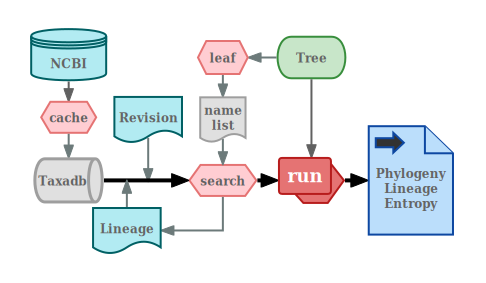
\includegraphics[width=0.9\textwidth]{CollapseWorkflow-Small.pdf}
	\caption{The Basic Workflow of CLTree. The red blocks are the token of cltree, and other blocks indicate the input/output files.}
	\label{workflow}
\end{figure}

The easiest way for preparing lineage information is utilizing the NCBI Taxonomy database dump file package directly. The file can be downloaded from the NCBI website (\url{https://ftp.ncbi.nlm.nih.gov/pub/taxonomy/taxdump.tar.gz}). With NCBI taxonomy dump file package and Tree.nwk, users can obtain the result by the command:
\begin{verbatim}
	cltree -i Tree.nwk -d taxdump.tar.gz
\end{verbatim}
In default mode, this command will output four files included annotated tree, lineage statisics, and Shannon entropy between phylogeny and lineage (see Table \ref{output})
\begin{table}[h]
  \caption{The defualt output files of cltree}
  \label{output}
  \centering
  \begin{tabular}{l p{0.6\textwidth}}
  \hline\hline
  file name & description \\
  \hline
  collapsed.entropy  & the Shannon entropy for every taxon rank \\
  collapsed-annotated.nwk & a newick tree with every node annotated with the common lineage for all sub branches \\
  collapsed.lineage & lineages for all genomes in CSV format\\
  collapsed.unit & stastistics for all taxon ranks in the rank order\\
  \hline\hline
  \end{tabular}
\end{table}

And to speedup, users can make the cache for the NCBI taxonomy database package by using the  command:
\begin{verbatim}
  cltree cache -d taxdump.tar.gz 
\end{verbatim}
The command will generate a cache file for the database dump, named ``taxadb.gz''. It will speedup the program in future tasks.



\subsection{Lineage Information Preparation}

There are two formats for recording the lineage information, i.e. CSV and custom format. The simple way is using the CSV format. It records one lineage information of a genome per line, with the taxon rank at the header (see the lineage.csv in the example folder of source code). 

\subsection{Advance Lineage Tools}
There are two columns in this file. The first column is the name of the species, and the lineage is shown in the second column

\begin{verbatim}
  superkingdom    D
  kingdom         K
  subkingdom      k
  superphylum     Q
  phylum          P
  subphylum       p
  superclass      L
  class           C
  subclass        c
  superorder      W
  order           O
  suborder        o
  family          F
  subfamily       f
  genus           G
  subgenus        g
  species         S
  subspecies      s
  \end{verbatim}
  

\begin{itemize}
	\item Example of lineage file:
{\footnotesize
\begin{verbatim}
Chlamydia_pecorum_...RefSeq <D>Bacteria<P>Chlamydiae...<S>Chlamydia_pecorum
Chlamydia_trachomatis...RefSeq <D>Bacteria<P>Chlamydiae...<S>Chlamydia_trachomatis
Chlamydia_pecorum...RefSeq  <D>Bacteria<P>Chlamydiae...<S>Chlamydia_pecorum
Chlamydia_trachomatis...RefSeq  <D>Bacteria<P>Chlamydiae...<S>Chlamydia_trachomatis
Corynebacterium_jeikeium...  <D>Bacteria<P>Actinobacteria...<S>Corynebacterium_jeikeium
Leptospira_interrogans...RefSeq <D>Bacteria<P>Spirochaetes...<S>Leptospira_interrogans
\end{verbatim}
}
\item Example for abbreviation of taxon ranks
\end{itemize}
A Example for batch revision
{\footnotesize
\begin{verbatim}
# Phylum B13 Firmicutes
<F>Erysipelotrichaceae<G>Eubacterium <F>Erysipelotrichaceae<G>Erysipelothrix   # CVTree
<P>Firmicutes<C>Erysipelotrichia <P>Tenericutes<C>Erysipelotrichia  # CVTree
<F>Unclassified<G>Exiguobacterium <F>Bacillaceae<G>Exiguobacterium   # CVTree
<F>Planococcaceae<G>Solibacillus <F>Bacillaceae<G>Solibacillus  #   NCBI taxonomy -> LPSN
\end{verbatim}
}


\section{Command Usage}
\subsection{Basic Usage}
To obtain a basic usage of the program and tasks, you can use the ``help" token, as {\tt cltree help} or {\tt cltree -h}. The output of the help information is shown in below. And users can type {\tt cltree help Task} to get more information about other tasks.

\begin{verbatim}
cltree Task [options]
 Available Task:
   run       Annotate phylogenetic tree with lineage system
   cache     Make NCBI database cache from taxdump.tar.gz
   query     Query lineage from local NCBI taxonomy database
   search    Search lineage from lineage files and NCBI taxonomy
             database, and revised by the revision file
   leaf      Obtain the species name list of phylogenetic tree
   rank      Output the default rank names and abbreviations
   help      Provide the help information for <Task>
 [ -h ]      Display this information
\end{verbatim}

\subsection{Default Task}
{\tt cltree run} perform the main task annotating phylogenetic tree by lineage and measuring their Differences by Shannon entropy. Due to this is the default task of the command, the token {\tt run} can be omitted except for the ``-h'' option. 
\begin{verbatim}
cltree run
 [ -D ./ ]              The work directory, default: ./
 [ -i Tree.nwk ]        Input newick tree, default: Tree.nwk
 [ -o collapsed ]       Output prefix name: default: collapsed
 [ -m <Revision.txt> ]  Lineage revision file for batch edit,
                        default: None
 [ -l Lineage.txt ]     Lineage file for leafs of tree,
                        default: Lineage.txt or Lineage.csv
 [ -d taxadb.gz ]       Taxa database file or directory,
                        default: taxadb.gz or taxdump.tar.gz
 [ -R <None> ]          List of rank names and abbreviations,
                        default: use the setting of program
 [ -r DKPCOFGS ]        Abbreviation of output taxon rank,
                        default: according to source
 [ -O <Outgroup> ]      Set the outgroup for the unroot tree.
                        default: None, rearranged by taxonomy
 [ -P ]                 Output prediction for undefined leafs
 [ -q ]                 Run command in quiet mode
 [ -h ]                 Display this information
 \end{verbatim}

\subsection{Lineage Tasks}
Users can also obtain the leaf lineages of the phylogenetic tree by other task step by step and review them manually, i.e. using {\tt cltree leaf} obtain the name list of phylogenic tree, and using {\tt cltree search} obtain the lineages of the speceis. The function and usage of these two programs are shown below: 
 
\begin{itemize}\itemsep 0pt 
  \item leaf -- Obtain the name list of phylogenetic tree
  \begin{verbatim}
  cltree leaf
   [ -i Tree.nwk ]      Input tree file, default: Tree.nwk
   [ -o namelist.txt ]  Output name list, default: name.list
   [ -q ]               Run command in quiet mode
   [ -h ]               Display this information
  \end{verbatim}

\item search -- Search the lineage of the genome
\begin{verbatim}
cltree search
 [ -i namelist.txt ]    Input name list, ':N' after the file name
                        select the N column of the file
                        default: first column of namelist.txt
 [ -o Lineage.csv ]     Output lineage file, default: lineage.csv
 [ -m <Revision.txt> ]  Lineage revise file for batch edit,
                        default: None
 [ -l Lineage.txt ]     Lineage file for leafs of tree,
                        default: Lineage.txt
 [ -d taxadb.gz ]       Taxa database file or directory,
                        default: taxadb.gz or taxdump.tar.gz
 [ -R <None> ]          List file for rank names and abbreviations,
                        default: use the setting of program
 [ -r <DKPCOFGS> ]      Set output taxon rank by abbreviations,
                        default: according to source
 [ -q ]                 Run command in quiet mode
 [ -h ]                 Display this information
\end{verbatim}
\end{itemize}

\subsection{NCBI Taxonomy Database Tasks}
Other tasks of the program are used to handle the NCBI Taxonomy database.

\begin{itemize}
\item cache -- Package the dump files of NCBI taxonomy database as cache to speed up query lineage from database.
  \begin{verbatim}
  cltree cache
   [ -d taxdump.tar.gz ]  NCBI taxon dumpfile directory, default: taxdump.tar.gz
   [ -o taxadb.gz ]       Packaged taxon database, default: taxadb.gz
   [ -q ]                 Run command in quiet mode
   [ -h ]                 Display this information
  \end{verbatim}

\item rank -- Output an example for the ordered list of the taxon rank names and abbreviations.
\begin{verbatim}
cltree rank
 [ -o ranklist.txt ]  Output name list, default: ranklist.txt
 [ -q ]               Run command in quiet mode
 [ -h ]               Display this information
\end{verbatim}

\item query -- Query the lineage of the genome ONLY from NCBI Taxonomy database dump files or the database cache.
\begin{verbatim}
cltree query
 [ -I <Taxon ID> ]     Query a taxon id
 [ -N <Taxon Name> ]   Query a taxon name
 [ -i namelist.txt ]   The query list file default: name.list
 [ -d taxadb.gz ]      The dump of NCBI taxonomy database
 [ -o Lineage.txt ]    Output file, default: Lineage.txt
 [ -R <None> ]         List file for rank names and abbreviations,
                       default: use the setting of program
 [ -r <DKPCOFGS> ]     Set output taxon rank by abbreviations,
                       default: same to the source
 [ -H ]                Don't output missing items
 [ -q ]                Run command in quiet mode
 [ -h ]                Display this information
\end{verbatim}
\end{itemize}

\section{Algorithm}

\subsection{Annotate the Phylogeny Tree}
	
\subsection{Measure Difference by Shannon Entropy}


\section{Citing Collapse in a Publication}
Please cite:
\begin{enumerate}\itemsep 0pt
	\item Guanghong Zuo (2021) Collapse: Annotate Phylogenetic Tree by Lineage and Measure their Differences by Shannon Entropy. {\tt in preparation}.
\end{enumerate}

\addcontentsline{toc}{section}{Reference}
\begin{thebibliography}{}
	\bibitem[Zuo, 2021]{z20}
	Zuo, G. (2021) Collapse: Annotate Phylogenetic Tree by Lineage and Measure their Differences by Shannon Entropy. \newblock {\em Journal}, {\tt in submission}.
\end{thebibliography}
\end{document}
